\chapter{Training TODO: change name, kinda cringe}
\section{Reaching a static target}
\subsection{The Problem} \label{static_target:the_problem}
A common task for an AI in a game is to reach a a given destination. According to \cite{alonso2020deeplearningnavigation} the common way to achieve this goal is by using \emph{navigation meshes} (NavMeshes). These are represented as graphs, and their nodes represent surfaces that can be traversed. Afterwards, algorithms such as \emph{A*} can be used to find the fastest way for an agent to go from point A to point B. However, these \emph{NavMeshes} require to be \emph{baked} (TODO explicatie baked) in advance, so updating them in real time can prove to be a challenge depending on several factors such as:
\begin{itemize}
    \item the game engine used
    \item the complexity of the game environment
    \item the computational cost associated with recreating in real time these meshes
\end{itemize}

A proposed solution for this problem would be to use AI agents that have been trained using deep learning methods, in such a manner that they would be independent from changes to the environment.

\subsection{Implementing the solution} \label{static_target:implementation}
\paragraph{}
First, the action space for the agent is defined: due to the fact that we only need to move the agent to a given position, the action space consists of moving the agent forward or backward, and rotating it. Because the agent is supposed to be controlled by a controller, its movement input is defined as a real number in the $[-1, 1]$ interval for both $X$ and $Y$ axes. However, a discrete action space will be used instead of a continuous one to reduce the difficulty of learning, and also because there is no need for the agent to have movements that are so precise. For each axis the action space will be represented by the discrete space: $\{-1, -0.5, 0, 0.5, 1\}$.

\paragraph{}
To make decisions, the agent will need to make several observations about its surroundings. Firstly, it will need to know how close it is to certain objects in the environment. To accomplish this, several \emph{raycasts} will be used to measure the distance from the agent, similar to a \emph{LIDAR} (TODO: add ceva despre lidar si un paper). The raycasts start from the center of the agent and are spread in such a way that the angle between 2 consecutive rays is equal for any 2 consecutive rays (TODO: imagine cu rays, si probabil sa gasesc un termen mai ok). The observation will contain the distance until the rays hit an object. Also, the index of the layer of the hit object will be included in the observations, so that the agent will differentiate between regular environment objects and more important objects, such as other players, enemies, etc. For this implementation, 32 rays were used.

Other observations that are made are the agent's position in space and also that of the target. This observation is included so that the agent can learn how movement brings it closer or further to the target. The next observation is the agent's forward vector so it can know in which direction it is moving. The optimal direction that the agent should take is also observed and obtained by computing the vector difference between the target's position and the agent's position. To know how much to adjust its trajectory, the angle between the agent's forward vector and the target is observed; the angle is signed so that the agent can learn to adjust its trajectory to the left or to the right. The distance to the target is added to the observations so that the agent can learn that when the distance is getting smaller it is rewarded. The agent's normalized velocity vector is observed to show in which direction it is moving based on the given input. The angle between the agent's velocity vector and its forward vector is observed to tell if the agent is moving forwards or backwards. Finally, the agent's velocity magnitude is observed so the agent can know if it is moving or standing still. 

In summary the following observations are being made:
\begin{itemize}
    \item distance for each raycast until it hits an object
    \item layer index of object hit by the raycast
    \item spatial postion of the agent
    \item spatial position of the target
    \item agent's forward vector
    \item optimal direction of the agent
    \item signed angle between the agent's forward vector and the target
    \item distance from the target
    \item agent's normalized velocity vector
    \item angle between the agent's velocity vector and its forward vector
    \item agent's velocity magnitude
\end{itemize}

\paragraph{}
In order for the agent to be able to learn to solve a specific problem, in this case, to reach a target, it must be rewarded or punished according to the actions that were taken. It is important to be mindful of the rewards that are given to the agent because only giving rewards and not punishing it can lead the agent to learn a behaviour that will maximize its reward, but will not be able to solve the problem, as it will be described shortly.

To begin, the first reward that was implemented, was the reward for reaching the objective, which is the goal of the agent and should also be a substantial reward. The other rewards that ware added were based on the direction of the movement and how close to the target it was, the reward increasing in value if the agent was closer to the objective (\ref{reward:1}) and a reward if the raycasts are hitting the destination object, which also increases in value if the agent is closer to the target (\ref{reward:2}). 

\begin{equation} \label{reward:1}
    R = \frac{(1 - \frac{\alpha}{180}) \cdot r}{d}
\end{equation}
where:
\begin{itemize}
    \item [$R$]: is the total reward
    \item [$\alpha$]: is the angle between the agent's current direction and the optimal direction
    \item [$r$]: is the reward that is obtained if the agent has the optimal direction
    \item [$d$]: is the distance from the agent to the objective
\end{itemize}

\begin{equation} \label{reward:2}
    R = \frac{r}{d_{i}}
\end{equation}
where:
\begin{itemize}
    \item [$R$]: is the total reward
    \item [$r$]: is the reward obtained if the distance between the agent and the objective is minimum
    \item [$d_{i}$]: is the obtained distance by the raycast $i$ from the agent to the object
\end{itemize}

However, these three rewards are not enough for the agent: through learning experiments it was observed that the agent was performing poorly: it would get stuck trying to move through a wall, it would never reach the objective and just spin around, or in some cases, it would just stand still.

To solve these problems, several punishments were implemented to correct the behavior of the agent. To prevent the agent for not moving, a constant penalty was added, to incentivise the agent to move towards the reward, so that it will receive a reward. Also, to comabat standing still, if the agent does not move, it receives an additional penalty, and if it does not move for more than 100 time steps, it receives a huge penalty and the episode ends. 

To stop the agent from trying to pass thorugh walls, a penalty is added if the raycasts that hit walls or other objects in the environment, have the distance to the hit object be a smaller than a given number. This penalty also increases the closer the agent gets to a wall (\ref{punishment:1}). 

\begin{equation} \label{punishment:1}
    R = \frac{p}{d_{i}}, \text{if } d_{i} < d
\end{equation}
where:
\begin{itemize}
    \item [$R$]: is the total reward
    \item [$p$]: is the penalty obtained if the distance between the agent and the wall/environmental object is minimum
    \item [$d_{i}$]: is the obtained distance by the raycast $i$ from the agent to the object
    \item [$d$]: is the maximum distance for which the penalty is applied
\end{itemize}

Another penalty was added if the agent is moving away from objective, and as before, it increases the further away it gets from the objective (\ref{punishment:2}). 

\begin{equation} \label{punishment:2}
    R = \frac{\alpha}{180} \cdot p
\end{equation}
where:
\begin{itemize}
    \item [$R$]: is the total reward
    \item [$p$]: is the penalty obtained if the distance between the agent and the wall/environmental object is minimum
    \item [$\alpha$]: is the angle between the agent's current direction and the optimal direction
\end{itemize}

Through training, two undesirable behaviours were observed: it was observed that the agent would sometimes make sudden jerky movments, trying to change its direction and immediatly returning to its previous trajectory, and that the agent would learn to drive backwards. To fix the first problem, a penalty was added if the agent would change its direction (\ref{punishment:3}), and to fix the second one, a penalty was added if the tank was moving backwards (\ref{punishment:4}).

\begin{equation} \label{punishment:3}
    R = \frac{\alpha}{180} \cdot p
\end{equation}
where:
\begin{itemize}
    \item [$R$]: is the total reward
    \item [$p$]: is the penalty obtained for changing the movement direction
    \item [$\alpha$]: is the angle between the agent's current direction and its previous direction
\end{itemize}

\begin{equation} \label{punishment:4}
    R = \frac{\alpha}{180} \cdot p, \text{if } \alpha > 90
\end{equation}
where:
\begin{itemize}
    \item [$R$]: is the total reward
    \item [$p$]: is the penalty obtained for changing the movement direction
    \item [$\alpha$]: is the angle between the agent's current direction and its forward vector
\end{itemize}

In summary, the used rewards and penalites and their values can be seen in table \ref{reward_punish_table:1}

\begin{table}
    \centering
    \begin{tabular}{|| m{15em} | m{4em} | m{15em} ||}
    \hline \hline
    \strong{Name} & \strong{Value} & \strong{Notes} \\ \hline \hline
    Reach Objective Reward & 10 &  \\ \hline
    Move Towards Objective Reward & 0.001 & is scaled by the distance between agent and objective \\ \hline
    Raycast Touches Objective Reward & 0.001 & is scaled by the distance between agent and objective \\ \hline
    Constant Penalty & -0.005 & is applied at each time step \\ \hline
    Not Moving Penalty & -0.05 &  \\ \hline
    Not Moving For 100 Steps Penalty & -50 &  \\ \hline
    Moving Towards Wall Penalty & -0.002 & is scaled by the distance between agent and object \\ \hline
    Moving Away From Objective Penalty & -0.025 & is scaled by the distance between agent and objective \\ \hline
    Sudden Movement Penalty & -0.01 & is scaled by the angle between the agent's current direction and its previous one \\ \hline
    Moving Backwards Penalty & -0.005 &  \\ \hline \hline
    \end{tabular}
    \caption{Rewards and Penalites}
    \label{reward_punish_table:1}
\end{table}

\subsection{Training} \label{static_target:training}

Each training session consisted of $10^7$ steps, and 30 agents were trained in parallel. The training times were between 3-4 hours. The agents are supposed to learn to reach an objective which appears in one of 17 predefined positions on the map. Once the agent reaches the objective, it is moved in another location chosen randomly. Each separate training instance uses the same seed for the random number generator, so that the objectives will appear in the same order for each of the training instances. Each training episode has a limit of $5000$ steps.

In the initial training sessions, the agents were unable to learn to reach the objective, becoming stuck rotating in a circle. A proposed solution was to keep the objective in the same position until the agent reaches it 30 times. After reaching the objective 30 times, the objective would start appearing in the random predefined locations. This was done to possibly kickstart the agent's learning process, but the approach failed, the agent being unable to learn to reach the objective. Another approach was to increase the neural network's size, however this approach prove unsuccessful as well. The approach that worked was to remove the agent's postion and the objective's position from the observations. TODO: sa zic de curiosity

The agent's training process was done using multiple neural network configurations, including different number of network layers ($1$, $3$, $5$, $7$) and different number of units per layer ($128$, $256$, $512$).

The hyperparameters used for the training were:
\begin{table}
    \centering
    \begin{tabular}{|| m{10em} | m{10em} ||}
        \hline \hline
        \strong{Hyperparameter} & \strong{Value} \\ \hline \hline
        Gamma & 0.9 \\ \hline
        Lambda & 0.95 \\ \hline
        Beta & 0.005 \\ \hline
        Epsilon & 0.2 \\ \hline
        Buffer Size & 8192 \\ \hline
        Batch Size & 256 \\ \hline
        Number of Epochs & 3 \\ \hline
        Learning Rate & 0.0003 \\ \hline \hline
    \end{tabular}
    \caption{Training hyperparameters}
    \label{static_target_hyperparameters}
\end{table}

\paragraph{}
The results for training the agent with 1 network layer can be seen in Figure \ref{train_results_static_1_layers}, and in Table \ref{move_to_static_targets_table:1}. In this case, the configuration with $256$ units was not able to be trained properly, remaining stuck moving in a circle. Between the two configurations that were successfully trained, it can be seen that the one with $128$ units, performed better during the training process than the one with $512$ units, obtaining, at the end, a mean reward that is higher by $18.79\%$.


\begin{figure}
    \begin{center}
        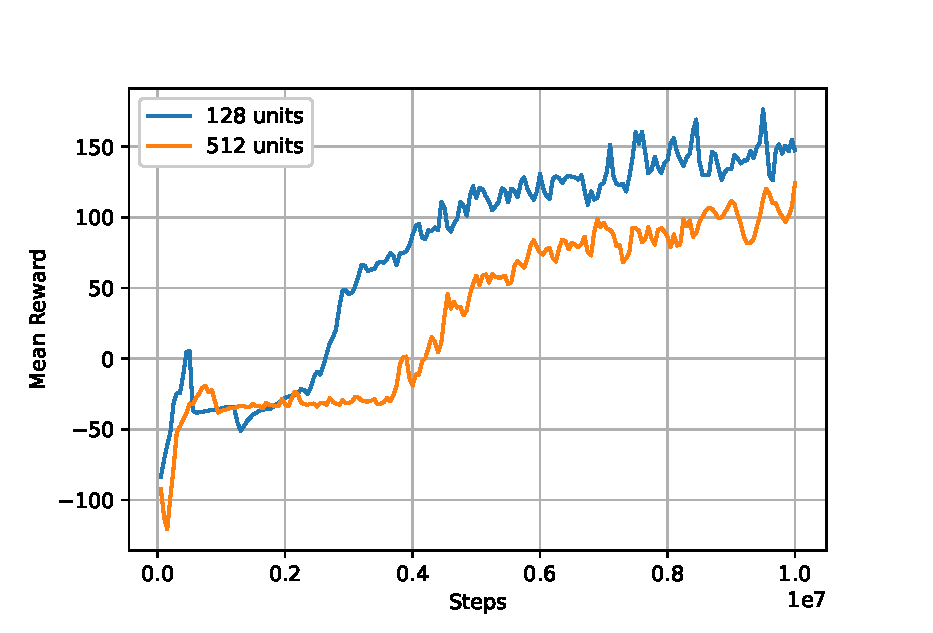
\includegraphics[width=0.95\linewidth]{move_to_static_target_1_layers.eps}
        \caption{Training results for reaching a static target with a network with 1 hidden layer}
        \label{train_results_static_1_layers}
    \end{center}
\end{figure}


% \paragraph{}
The results for training the agent with 3 network layers can be seen in Figure \ref{train_results_static_3_layers}, and in Table \ref{move_to_static_targets_table:1}. From these results, it can be seen that the configurations with $128$ and $256$ units, performed very similarily during the training, however, the one with $512$ units started to lag behind these two at around $4 \cdot 10^6$ steps. Again, the configuration with the least units had the best training results, obtaining a result that is $2.61\%$ better than the one with with $256$ units and better by $29\%$ than the one with $512$ units. 

\begin{figure}
    \begin{center}
        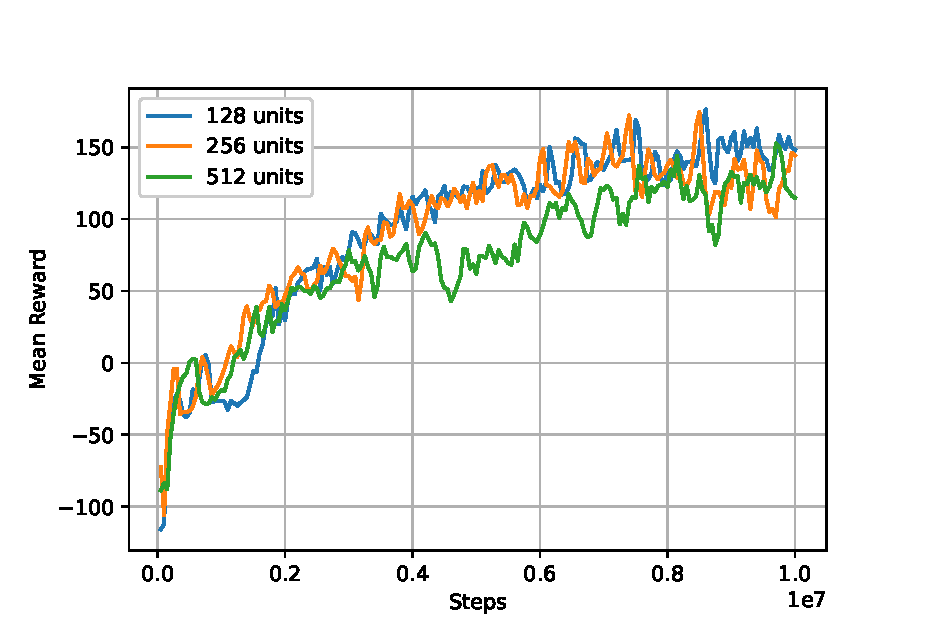
\includegraphics[width=0.95\linewidth]{move_to_static_target_3_layers.eps}
        \caption{Training results for reaching a static target with a network with 3 hidden layers}
        \label{train_results_static_3_layers}
    \end{center}
\end{figure}


% \paragraph{}
Results for training the agent with 5 network layers can be seen in Figure \ref{train_results_static_5_layers}, and in Table \ref{move_to_static_targets_table:1}. From the training results, it can be seen that in the later stages, the configuration with $256$ units falls behind the other two. Unlike the results with 1 layer and 3 layers, the best performing configuration is the one with $512$ units per layer, being better by $8.72\%$ than the configuration with $128$ units, and by $35.45\%$ than the configuration with $256$ units.

\begin{figure}
    \begin{center}
        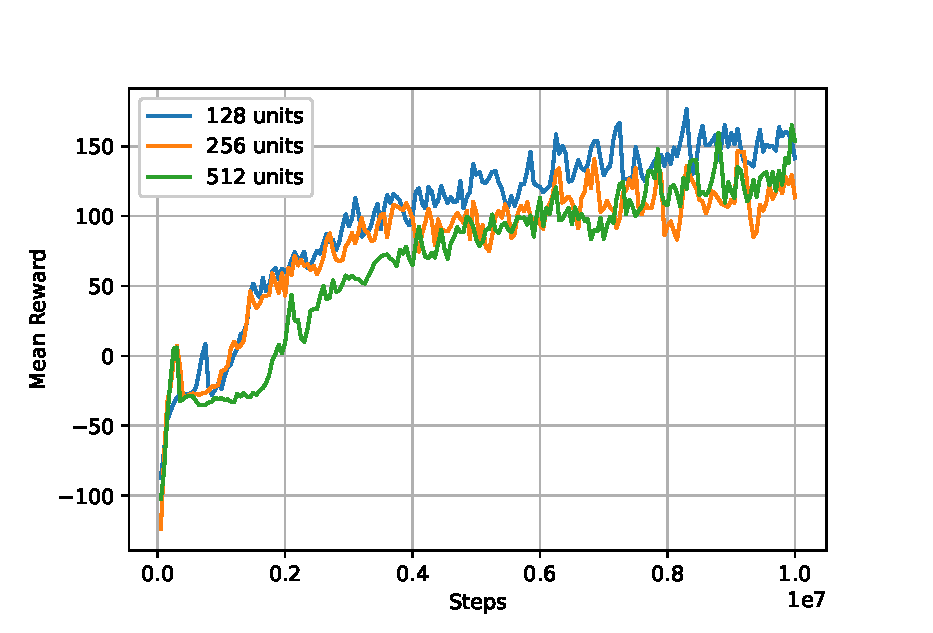
\includegraphics[width=0.95\linewidth]{move_to_static_target_5_layers.eps}
        \caption{Training results for reaching a static target with a network with 5 hidden layers}
        \label{train_results_static_5_layers}
    \end{center}
\end{figure}

% \paragraph{}
Results for training the agent with 7 network layers can be seen in Figure \ref{train_results_static_7_layers}, and in Table \ref{move_to_static_targets_table:1}. From the training results it can be seen that the configuration with $128$ units per layer performs better than the other two, but at the final stages of the training, it is caught up to by the configuration with $256$ units. In the end, the configurations with $128$ and $256$ units per layer had virtually identical results at the end of the training, and were better by $\sim36.3\%$ than the one with $512$ units.

\begin{figure}
    \begin{center}
        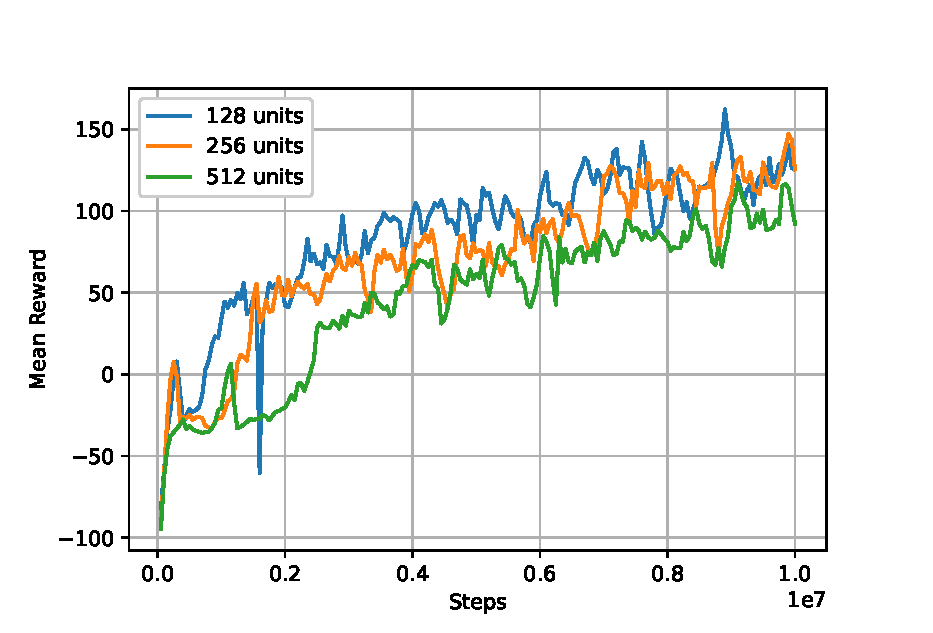
\includegraphics[width=0.95\linewidth]{move_to_static_target_7_layers.eps}
        \caption{Training results for reaching a static target with a network with 7 hidden layers}
        \label{train_results_static_7_layers}
    \end{center}
\end{figure}

\paragraph{}
All the training results can be seen in Table \ref{move_to_static_targets_table:1} and in Figure \ref{train_results_static_bar_chart}. It can be observed that network configurations with a smaller number of units per layer obtained better training results than the others. This could be due to the fact that the problem is not a very complex one, and because a smaller network can be trained faster. The configurations with 1, 3, or 5 layers obtained similar results, however, when 7 layers are used, there is a noticeable decrease in the agent's performance. These being said, from the training results it seems that using a network configuration with less layers and less units per layer offers almost the best result, thus it is the most practical one to be used, since it uses the least computing resources. Using larger networks should be done by training the agent for longer periods of time. However, it is possible when using a smaller network to obtain an unusable model, as was the case in this experiment using a network configuration with 1 hidden layer and 256 units per layer.

\begin{table}
    \centering
    \begin{tabular}{|| m{15em} | m{15em} ||}
    \hline \hline
    \strong{Network Configuration} & \strong{Final Mean Reward} \\ \hline \hline
    1 layer, 128 units & 147.568 \\ \hline
    1 layer, 256 units & DNF \\ \hline
    1 layer, 512 units & 124.221 \\ \hline
    3 layers, 128 units & 148.136 \\ \hline
    3 layers, 256 units & 144.366 \\ \hline
    3 layers, 512 units & 114.828 \\ \hline
    5 layers, 128 units & 141.369 \\ \hline
    5 layers, 256 units & 113.478 \\ \hline
    5 layers, 512 units & 153.709 \\ \hline
    7 layers, 128 units & 125.727 \\ \hline
    7 layers, 256 units & 125.441 \\ \hline
    7 layers, 512 units & 92.128 \\ \hline \hline
    \end{tabular}
    \caption{Final training results for reaching a static target}
    \label{move_to_static_targets_table:1}
\end{table}

\begin{figure}
    \begin{center}
        \includegraphics[width=\linewidth]{move_to_static_target_bar_chart.eps}
        \caption{Training results for all network configurations for reaching a static target}
        \label{train_results_static_bar_chart}
    \end{center}
\end{figure}



% =====================================



\section{Reaching a moving target}


\subsection{The Problem} \label{moving_target:the_problem}
Another standard behavior of an AI in videogames is to be able to chase a target, so that it can, maybe, perform a specific action once the object controlled by the AI is close enough to the target (TODO: sa mai dezvolt asta). A simple way to achieve this behavior would be to use a \emph{NavMesh} and periodically change the agent's destination. Compared to the problem described at \ref{static_target:the_problem}, the addition here is that the agent has to recompute its route at specified intervals.

\paragraph{}
Again, the proposed solution would be to use AI agents that are trained using deep learning methods.

\subsection{Implementing the solution} \label{moving_target:implementation}
The basic implementation for this problem is the same as the one described at \ref{static_target:implementation}, with the same observations, rewards and penalties being used. The addition would be to add an observation that is the direction in which the target is moving. This can be used by the agent to predict in which direction the target is moving and to eventually intercept it along its trajectory. Another idea would be to add recurrent memory (TODO: sa zic ce e recurrent memory) to the agent so that it can achieve this result in a more \enquote{natural} way.

\subsection{Training} \label{moving_target:training}
The training is similar to the process described at \ref{static_target:training}, with the same number of agents being trained at the same time, same number of steps, same hyperparameters (Table \ref{static_target_hyperparameters}), etc. 

Trying to add recurrent memory to the agent was a failure, the agent being unable to learn to chase the target, and getting stuck moving in a circle. This behaviour happened even when changing the recurrent network's hyperparameters \emph{sequence length} and \emph{memory size}. (TODO: maybe add some combinations)

Training this agent was done in 2 separate ways: one where the target's direction is not in the observations, and one where it is. The first round of training is done without the observation that was mentioned previously.

\paragraph{}
Results for training the agent with a single network layer and without the target's direction obsrevation can be seen in Figure \ref{train_results_moving_1_layers} and Table \ref{move_to_moving_targets_table:1}. From these results it can be seen that all 3 configurations performed virtually identically, and at the end of the training had obtained the same mean reward.

\begin{figure}
    \begin{center}
        \includegraphics[width=0.95\linewidth]{move_to_moving_target_1_layers.eps}
        \caption{Training results for reaching a moving target with a network with 1 hidden layer}
        \label{train_results_moving_1_layers}
    \end{center}
\end{figure}


Results for training the agent with 3 network layers and without the target's direction obsrevation can be seen in Figure \ref{train_results_moving_3_layers} and Table \ref{move_to_moving_targets_table:1}. In these results, it seems that the configuration with $128$ units obtains better results during training than teh configuration with $256$ units, which in turn obtains better results than the one with $512$ units. At the end of the training, the configuration with $128$ units is better by $1.02\%$ than the one with $256$ units and better by $28.58\%$ than the one with $512$ units.

\begin{figure}
    \begin{center}
        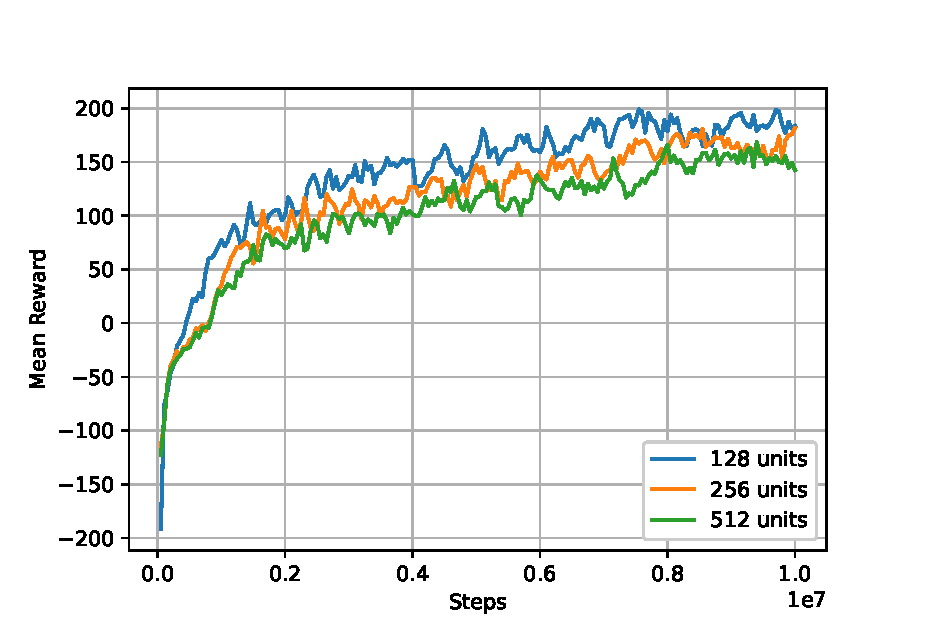
\includegraphics[width=0.95\linewidth]{move_to_moving_target_3_layers.eps}
        \caption{Training results for reaching a moving target with a network with 3 hidden layers}
        \label{train_results_moving_3_layers}
    \end{center}
\end{figure}


Results for training the agent with 5 network layers and without the target's direction obsrevation can be seen in Figure \ref{train_results_moving_5_layers} and Table \ref{move_to_moving_targets_table:1}. The results during training are similar to the configuration with 3 layers, with the configuration with $128$ units being better than the other two. The final result is that the configuration with $128$ units is better by $8.87\%$ than the one with $256$ units and better by $17.9\%$ than the one with $512$ units.

\begin{figure}
    \begin{center}
        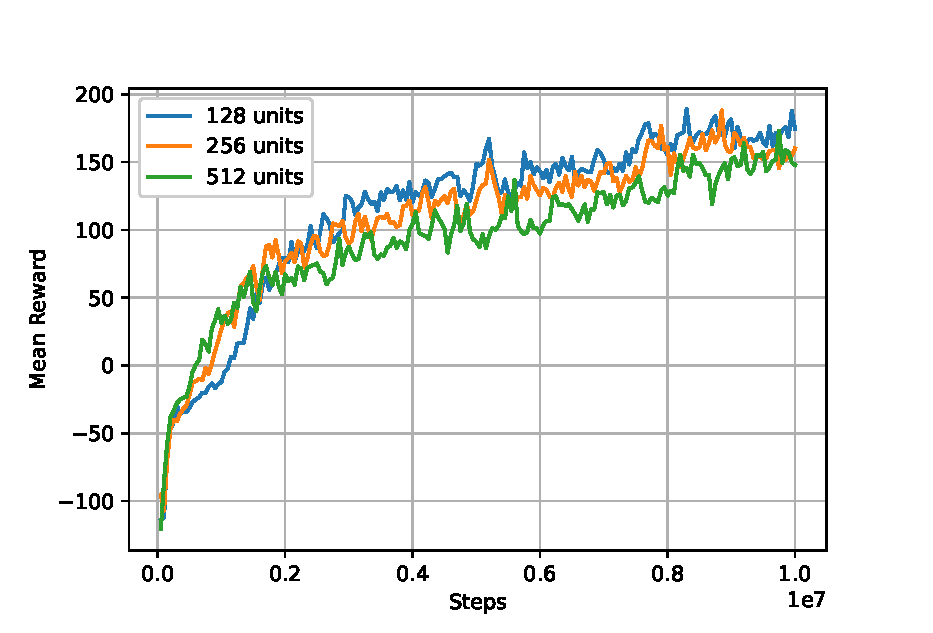
\includegraphics[width=0.95\linewidth]{move_to_moving_target_5_layers.eps}
        \caption{Training results for reaching a moving target with a network with 5 hidden layers}
        \label{train_results_moving_5_layers}
    \end{center}
\end{figure}


\paragraph{}
The second round of training is done by adding the target's movement direction to the agent's observations.

The results for training the agent with a single network layer and without the target's direction obsrevation can be seen in Figure \ref{train_results_moving_1_layers_with_dir} and Table \ref{move_to_moving_targets_table:1}.

\begin{figure}
    \begin{center}
        \includegraphics[width=0.95\linewidth]{move_to_moving_target_1_layers_with_dir.eps}
        \caption{Training results for reaching a moving target with a network with 1 hidden layer and with observation of target's direction}
        \label{train_results_moving_1_layers_with_dir}
    \end{center}
\end{figure}

\begin{figure}
    \begin{center}
        \includegraphics[width=0.95\linewidth]{move_to_moving_target_3_layers_with_dir.eps}
        \caption{Training results for reaching a moving target with a network with 3 hidden layers and with observation of target's direction}
        \label{train_results_moving_3_layers_with_dir}
    \end{center}
\end{figure}

\begin{figure}
    \begin{center}
        \includegraphics[width=0.95\linewidth]{move_to_moving_target_5_layers_with_dir.eps}
        \caption{Training results for reaching a moving target with a network with 5 hidden layers and with observation of target's direction}
        \label{train_results_moving_5_layers_with_dir}
    \end{center}
\end{figure}



\begin{table}
    \centering
    \begin{tabular}{|| m{11.3em} | m{10em} | m{9.6em} ||}
    \hline \hline
    \strong{Network Configuration} & \strong{Observed target's direction} & \strong{Final Mean Reward} \\ \hline \hline
    1 layer, 128 units & No & 184.547 \\ \hline
    1 layer, 128 units & Yes & 191.184 \\ \hline
    1 layer, 256 units & No & 184.563 \\ \hline
    1 layer, 256 units & Yes & 137.075 \\ \hline
    1 layer, 512 units & No & 185.936 \\ \hline
    1 layer, 512 units & Yes & 178.876 \\ \hline
    3 layers, 128 units & No & 183.288 \\ \hline
    3 layers, 128 units & Yes & 200.502 \\ \hline
    3 layers, 256 units & No & 181.435 \\ \hline
    3 layers, 256 units & Yes & 196.064 \\ \hline
    3 layers, 512 units & No & 142.54 \\ \hline
    3 layers, 512 units & Yes & 210.524 \\ \hline
    5 layers, 128 units & No & 174.404 \\ \hline
    5 layers, 128 units & Yes & 191.399 \\ \hline
    5 layers, 256 units & No & 159.966 \\ \hline
    5 layers, 256 units & Yes & 164.351 \\ \hline
    5 layers, 512 units & No & 147.922 \\ \hline
    5 layers, 512 units & Yes & 193.828 \\ \hline \hline
    \end{tabular}
    \caption{Final training results for reaching a moving target}
    \label{move_to_moving_targets_table:1}
\end{table}

\begin{figure}
    \begin{center}
        \includegraphics[width=\linewidth]{move_to_moving_target_bar_chart.eps}
        \caption{Training results for all network configurations for reaching a moving target}
        \label{train_results_moving_bar_chart}
    \end{center}
\end{figure}



% ===============================================



\section{Shooting a moving target}

\subsection{The Problem}



\subsection{Implementing the solution}




\subsection{Training}




\begin{figure}
    \begin{center}
        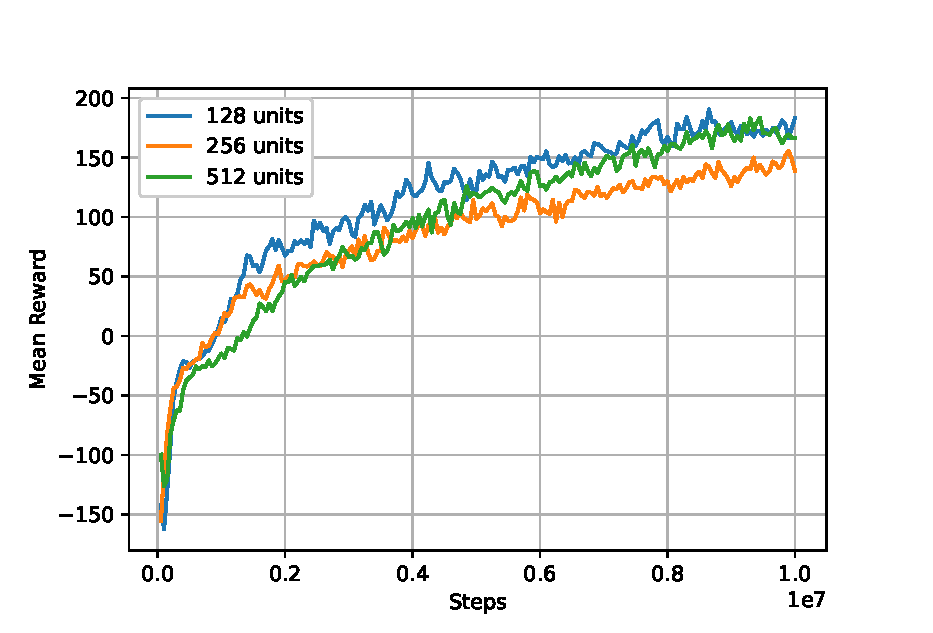
\includegraphics[width=0.95\linewidth]{shoot_moving_target_1_layers.eps}
        \caption{Training results for shooting a moving target with a network with 1 hidden layer}
        \label{train_results_shoot_1_layers}
    \end{center}
\end{figure}

\begin{figure}
    \begin{center}
        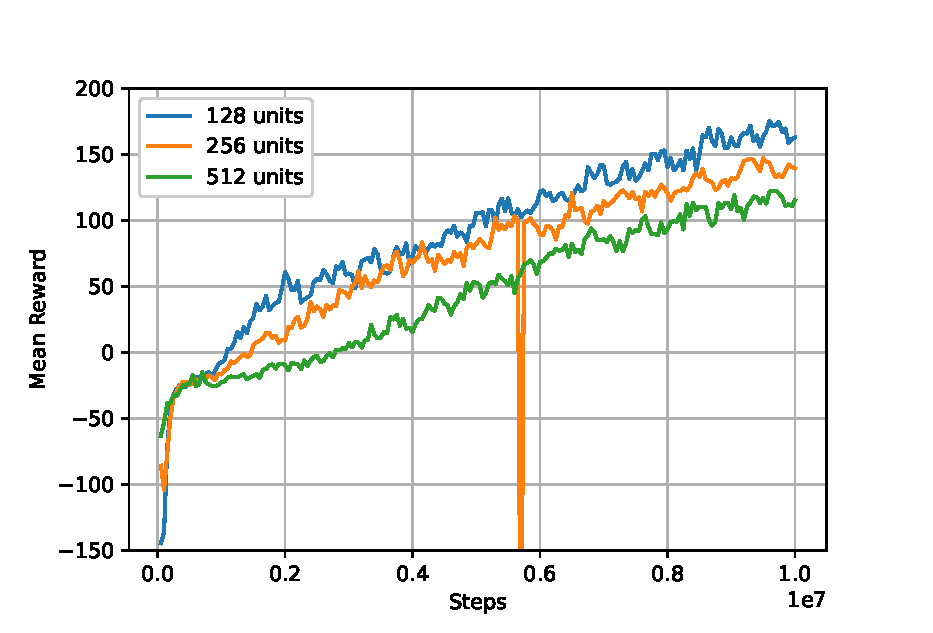
\includegraphics[width=0.95\linewidth]{shoot_moving_target_3_layers.eps}
        \caption{Training results for shooting a moving target with a network with 3 hidden layers}
        \label{train_results_shoot_3_layers}
    \end{center}
\end{figure}

\begin{figure}
    \begin{center}
        \includegraphics[width=0.95\linewidth]{shoot_moving_target_5_layers.eps}
        \caption{Training results for shooting a moving target with a network with 5 hidden layers}
        \label{train_results_shoot_5_layers}
    \end{center}
\end{figure}

\begin{figure}
    \begin{center}
        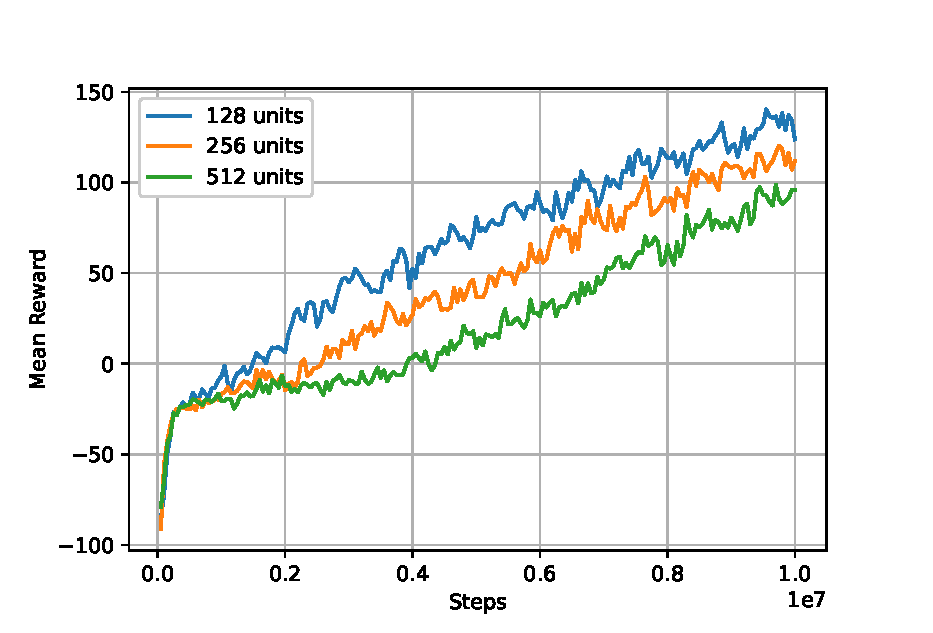
\includegraphics[width=0.95\linewidth]{shoot_moving_target_7_layers.eps}
        \caption{Training results for shooting a moving target with a network with 7 hidden layers}
        \label{train_results_shoot_7_layers}
    \end{center}
\end{figure}



\begin{figure}
    \begin{center}
        \includegraphics[width=0.95\linewidth]{shoot_moving_target_128_1_layers.eps}
        \caption{Training results for shooting a moving target with a network with 1 hidden layer, 128 units, and different observations}
        \label{train_results_shoot_obs_comparasion_1_layers}
    \end{center}
\end{figure}

\begin{figure}
    \begin{center}
        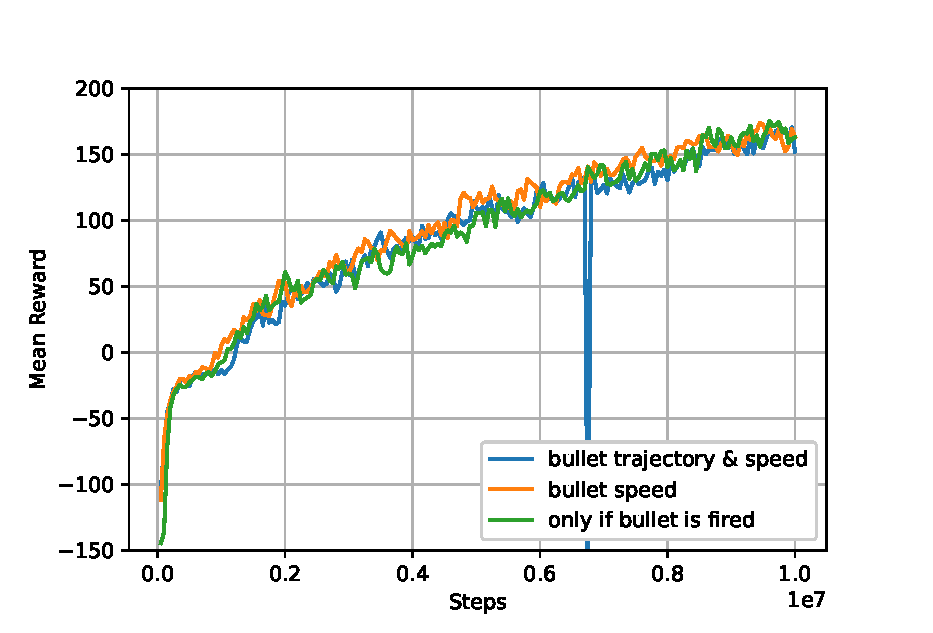
\includegraphics[width=0.95\linewidth]{shoot_moving_target_128_3_layers.eps}
        \caption{Training results for shooting a moving target with a network with 3 hidden layers, 128 units, and different observations}
        \label{train_results_shoot_obs_comparasion_3_layers}
    \end{center}
\end{figure}

\begin{figure}
    \begin{center}
        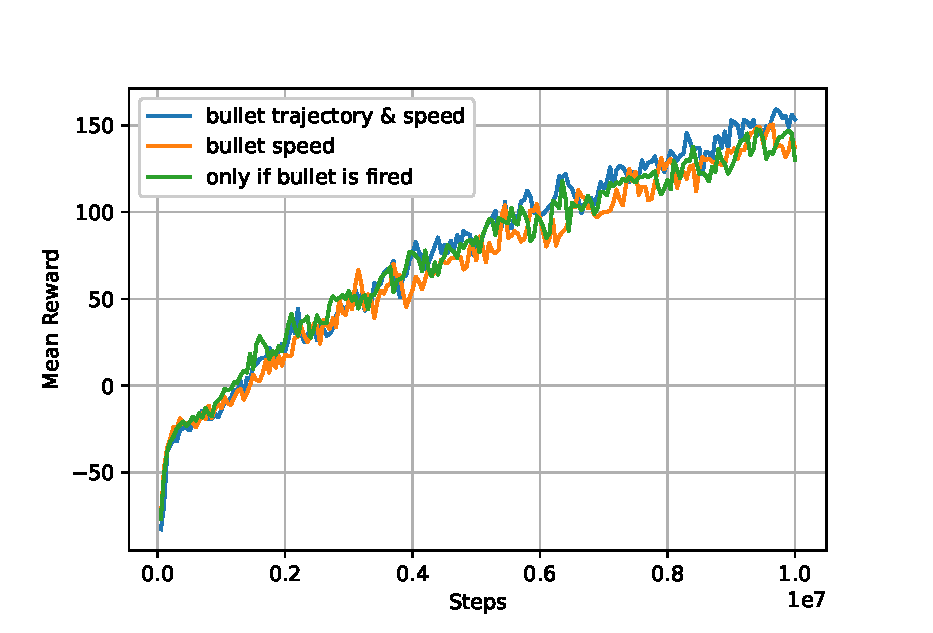
\includegraphics[width=0.95\linewidth]{shoot_moving_target_128_5_layers.eps}
        \caption{Training results for shooting a moving target with a network with 3 hidden layers, 128 units, and different observations}
        \label{train_results_shoot_obs_comparasion_5_layers}
    \end{center}
\end{figure}

\begin{figure}
    \begin{center}
        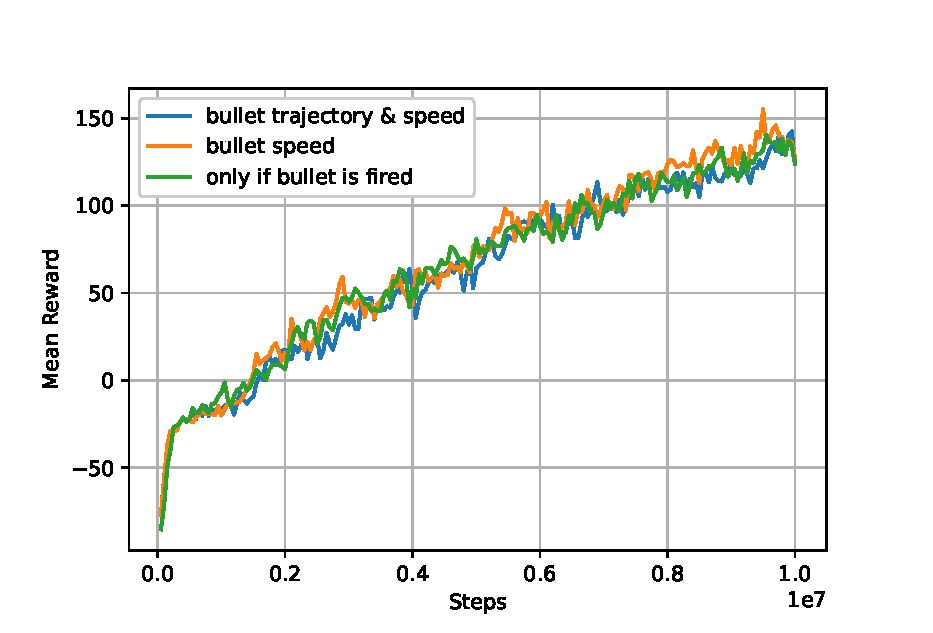
\includegraphics[width=0.95\linewidth]{shoot_moving_target_128_7_layers.eps}
        \caption{Training results for shooting a moving target with a network with 3 hidden layers, 128 units, and different observations}
        \label{train_results_shoot_obs_comparasion_7_layers}
    \end{center}
\end{figure}


\begin{table}
    \centering
    \begin{tabular}{|| m{15em} | m{15em} ||}
    \hline \hline
    \strong{Network Configuration} & \strong{Final Mean Reward} \\ \hline \hline
    1 layer, 128 units & 183.278 \\ \hline
    1 layer, 256 units & 138.719 \\ \hline
    1 layer, 512 units & 166.612 \\ \hline
    3 layers, 128 units & 162.629 \\ \hline
    3 layers, 256 units & 139.293 \\ \hline
    3 layers, 512 units & 115.129 \\ \hline
    5 layers, 128 units & 130.032 \\ \hline
    5 layers, 256 units & 127.781 \\ \hline
    5 layers, 512 units & 100.497 \\ \hline
    7 layers, 128 units & 123.777 \\ \hline
    7 layers, 256 units & 111.752 \\ \hline
    7 layers, 512 units & 95.882 \\ \hline \hline
    \end{tabular}
    \caption{Final training results for shooting a moving target}
    \label{shoot_moving_targets_table:1}
\end{table}

\begin{table}
    \centering
    \begin{tabular}{|| m{12em} | m{12em} | m{10em} ||}
    \hline \hline
    \strong{Network Configuration} & \strong{Bullet Observations} & \strong{Final Mean Reward} \\ \hline \hline
    1 layer, 128 units & Bullet's direction and speed & 156.766 \\ \hline
    1 layer, 128 units & Bullet's speed & 166.427 \\ \hline
    1 layer, 128 units & Only if bullet was fired & 183.278 \\ \hline
    3 layers, 128 units & Bullet's direction and speed & 152.188 \\ \hline
    3 layers, 128 units & Bullet's speed & 163.311 \\ \hline
    3 layers, 128 units & Only if bullet was fired & 162.629 \\ \hline
    5 layers, 128 units & Bullet's direction and speed & 153.46 \\ \hline
    5 layers, 128 units & Bullet's speed & 137.391 \\ \hline
    5 layers, 128 units & Only if bullet was fired & 130.032 \\ \hline
    7 layers, 128 units & Bullet's direction and speed & 125.061 \\ \hline
    7 layers, 128 units & Bullet's speed & 127.677 \\ \hline
    7 layers, 128 units & Only if bullet was fired & 123.777 \\ \hline \hline
    \end{tabular}
    \caption{Final training results for shooting a moving target with different bullet observations}
    \label{shoot_moving_targets_table:2}
\end{table}


\begin{figure}
    \begin{center}
        \includegraphics[width=\linewidth]{shoot_moving_target_bar_chart.eps}
        \caption{Training results for all network configurations for shooting a moving target}
        \label{train_results_shoot_bar_chart}
    \end{center}
\end{figure}

\begin{figure}
    \begin{center}
        \includegraphics[width=\linewidth]{shoot_moving_target_obs_comparasion_bar_chart.eps}
        \caption{Training results for network configurations with 128 units per layer and different bullet observations, for reaching a moving target}
        \label{train_results_shoot_obs_comparasion_bar_chart}
    \end{center}
\end{figure} 